\section{解析模板}

大多数编程语言的编译器的两个基本活动是标记化(也称为扫描或词法)和解析。标记化过程将源代码读取为字符序列,并从中生成一系列标记。例如,当看到字符序列int* p = 0;时,“分词器”会将为关键字int、符号/运算符*、标识符p、符号/运算符=、整数文字0和符号/运算符;生成记号描述。

然后,解析器通过递归减少标记或先前模式到更高级别的构造中,从而在标记序列中找到已知的模式。例如,词牌0是一个有效的表达式,后跟标识符p的组合*是一个有效的声明符,声明符后跟“=”再后跟表达式“0”是一个初始化声明符。最后,关键字int是已知的类型名称,当后跟初始化声明器*p = 0时,即得到p的初始化声明。

\subsection{非模板中的上下文相关性}

词法化比解析更容易,词法解析是一门已经发展出坚实理论的学科,许多语言都使用该理论进行解析。然而,该理论最适合上下文无关的语言,我们知道C++是上下文敏感的。为了处理这个问题,C++编译器会将符号表与分词器和解析器耦合起来:当解析一个声明时,会使用符号表进行解析。当分词器找到一个标识符时,会进行查找,并在找到匹配类型时对结果词法进行注释。

例如,C++编译器看到

\begin{cpp}
x*
\end{cpp}

分词器会查找x,如果找到类型,解析器将看到

\begin{cpp}
identifier, type, x
symbol, *
\end{cpp}

并得出结论说,这是一个声明。但是,如果x不是类型,则解析器从分词器接收到的信息为

\begin{cpp}
identifier, nontype, x
symbol, *
\end{cpp}

该构造只能通过乘法进行有效解析,这些细节取决于具体实现策略。

下面的表达式说明了上下文相关的另一个例子:

\begin{cpp}
X<1>(0)
\end{cpp}

如果X是类模板的名称,表达式将整数0强制转换为从该模板生成的类型X<1>。如果X不是模板,则表达式等价于

\begin{cpp}
(X<1)>0
\end{cpp}

换句话说,X与1比较,比较的结果(下隐式转换为1或0)与0比较。虽然这样的代码很少使用,但它是有效的C++(和有效的C)代码。因此,C++解析器将查找出现在<之前的名称,当知道该名称是模板名称时,才将<作为尖括号处理;否则,<将视为小于操作符。

这种形式的上下文相关性,是选择尖括号来分隔模板参数列表的结果。这是另一种情况:

\begin{cpp}
template<bool B>
class Invert {
public:
	static bool const result = !B;
};

void g() {
	bool test = Invert<(1>0)>::result; // parentheses required!
}
\end{cpp}

如果省略了Invert<(1>0)>中的圆括号,则大于符号将误认为模板参数列表的结束符号。这将使代码无效,因为编译器将其视为((Invert<1>))0>::result。

\begin{notice}
使用双括号是为了避免将(Invert<1>)0作为强制转换操作进行解析——这也是导致语法歧义的另一个原因。
\end{notice}

分词器也不能避免尖括号表示法的问题。例如:

\begin{cpp}
List<List<int>> a;
			 // ^ -- no space between right angle brackets
\end{cpp}

两个>字符组合成右移标记>{}>,因此分词器不会将其视为两个单独的标记。这是最大蒙克标记化原则的结果:C++实现必须将尽可能多的连续字符收集到标记中。

\begin{notice}
可以引入了特定的异常来解决本节中描述的标记化问题。
\end{notice}

正如在2.2节中提到的,C++11标准特别调用了这种情况——嵌套的模板标识使用>{}>标记作为结束——在解析器中,等同于两个独立的尖括号,一次性关闭两个模板。

\begin{notice}
1998年和2003年版本的C++标准不支持这种“尖括号黑客”。然而,需要在两个连续的尖括号之间加入一个空格,这对模板初学者来说是一个障碍,因此委员会决定在2011年的标准中对这种写法进行改变。
\end{notice}

这一变化改变了某些程序(诚然,这些程序是人为设计的)的意义。考虑下面的例子:

\filename{details/anglebrackethack.cpp}
\begin{cpp}
#include <iostream>

template<int I> struct X {
	static int const c = 2;
};

template<> struct X<0> {
	typedef int c;
};

template<typename T> struct Y {
	static int const c = 3;
};

static int const c = 4;

int main() {
	std::cout << (Y<X<1> >::c >::c>::c) << ' ';
	std::cout << (Y<X< 1>>::c >::c>::c) << '\n';
}
\end{cpp}

这是一套C++98代码,输为出0 3。在使用C++11标准时,尖括号使用方式的变革使得括号内的两个语句等价,所以输出为0 0。

\begin{notice}
一些提供C++98或C++03模式的编译器会保持C++11在这些模式下的行为,因此即使使用C++98/C++03编译也会打印0 0。
\end{notice}

由于"<:"是"["(在一些传统键盘上不可用)的替代,因此也存在类似的问题。看看下面的例子:

\begin{cpp}
template<typename T> struct G {};
struct S;
G<::S> gs; // valid since C++11, but an error before that
\end{cpp}

C++11前,最后一行代码相当于G[:S> gs;,这显然是无效的代码标识。为了解决这个问题,添加了另一个“词法黑客”:当编译器看到字符<::没有立即跟在:或>后面时,前导“<:”不再等同于“[”。

\begin{notice}
这是前面提到的最大蒙克原则的一个例外。
\end{notice}

这个黑客技巧使得以前有效(但有些人为)的代码,编程无效代码:

\begin{cpp}
#define F(X) X ## :

int a[] = { 1, 2, 3 }, i = 1;
int n = a F(<::)i]; // valid in C++98/C++03, but not in C++11
\end{cpp}

要理解这一点,“词法黑客”适用于预处理标记,这是预处理程序可以接受的标记类型(在预处理完成后可能无法接受),它们在宏展开完成之前决定。考虑到这一点,C++98/C++03在宏调用F(<::)中无条件地将“<:”转换为“[”,n的定义扩展为

\begin{cpp}
int n = a [ :: i];
\end{cpp}

这完全没问题。因为在宏展开之前,"<::"后面不是":"或">",而是")",所以C++11则不会进行字符转换。没有转换,连接操作符必须尝试将"::"和":"粘合到新的预处理标记中。但这不起作用,因为":::"不是有效的连接标记。C++11标准导致了这种未定义行为,有些编译器会诊断这个问题,只是将两个预处理标记分开,这是一个语法错误,因为它导致n的定义扩展为

\begin{cpp}
int n = a < :: : i];
\end{cpp}

\subsection{依赖型类型名称}

模板名称的问题在于,不能进行合理的分类。特别是,模板不能看到另一个模板,因为另一个模板的内容可以通过显式特化使其无效:

\begin{cpp}
template<typename T>
class Trap {
	public:
	enum { x }; // #1 x is not a type here
};

template<typename T>
class Victim {
	public:
	int y;
	void poof() {
		Trap<T>::x * y; // #2 declaration or multiplication?
	}
};

template<>
class Trap<void> { // evil specialization!
	public:
	using x = int; // #3 x is a type here
};

void boom(Victim<void>& bomb) {
	bomb.poof();
}
\end{cpp}

当编译器解析\#2行时,必须判断看到的是声明还是乘法,这取决于依赖的限定名Trap<T>::x是否是类型名。可能很容易在模板Trap中查找,并根据\#1行,知道Trap<T>::x不是一个类型,这将使\#2行是一个乘法,但其为T为void的情况重写了通用的Trap<T>::x。这种情况下,Trap<T>::x实际上是int类型。

例子中,类型Trap<T>是一个依赖类型,该类型依赖于模板参数T。而且,Trap<T>引用了一个未知的特化(在第13.2.4节中描述),从而编译器不能安全地查看模板内部,来确定名称Trap<T>::x是否是一个类型。如果"::"前面的类型引用当前实例化类——Trap<T>::y——编译器就可以看到模板定义,从而确定没有其他特化介入。因此,当"::"前面的类型指向当前实例化类时,模板中的限定名查找与非依赖类型的限定名查找非常类似。

但对未知特化的名称查找仍是一个问题。解决问题的方法是,指定依赖的限定名不表示类型,除非该名称以关键字typename作为前缀。若替换模板参数之后,发现名称不是类型的名称,则程序无效,并且C++编译器应该在实例化时报错。注意,typename的这种用法与表示模板类型参数的用法不同。与类型参数不同,不能等价地将typename替换为class。

当名称满足以下条件时,typename前缀是必需的:

\begin{notice}
C++20在大多数情况下可能会删除对typename的需要(请参阅第17.1节了解详细信息)。
\end{notice}

\begin{enumerate}
\item 
是有限定的,而不是在后面添加"::"形成一个更有限定的名称。

\item 
不是详细类型说明符(即以关键字class、struct、union或enum之一开头的类型名)的一部分。

\item 
不在基类规范列表中或引入构造函数定义的成员初始化式列表中使用。

\begin{notice}
[colback=webgreen!5!white,colframe=webgreen!75!black]
从语法上讲,这些上下文中只允许使用类型名,因此可以假设使用限定名来命名类型。
\end{notice}

\item 
依赖于模板参数。

\item 
是未知特化的成员,由限定符命名的类型指向未知的特化类型。
\end{enumerate}

此外,若不满足前两个条件,则不可使用typename前缀。为了说明这一点,看看以下的错误例子:

\begin{notice}
改编自[VandevoordeSolutions],多次证明C++代码重用的重要性。
\end{notice}

\begin{cpp}
template<typename1 T>
struct S : typename2 X<T>::Base {
	S() : typename3 X<T>::Base(typename4 X<T>::Base(0)) {
	}
	typename5 X<T> f() {
		typename6 X<T>::C * p; // declaration of pointer p
		X<T>::D * q; // multiplication!
	}
	typename7 X<int>::C * s;
	
	using Type = T;
	using OtherType = typename8 S<T>::Type;
};
\end{cpp}

每次出现typename(不管正确与否)都用一个下标进行编号,以便于引用。第一个typename$_1$表示模板参数。前面的规则不适用于第一次使用。

前面规则中的第二项不允许使用第二个和第三个类型名。这两个上下文中基类的名称之前不能有typename。但是,typename$_4$是必需的。这里,基类的名称不表示要初始化或派生的对象,而该名称是表达式的一部分,该表达式从其参数0构建临时X<T>::Base(可以认为是一种转换)。禁止使用第五个typename,因为后面的名称X<T>不是限定名称。若此语句要声明指针,则typename需要出现第六次。下一行省略了typename关键字,因此编译器将其解释为乘法。第七个typename可选,因为它满足前两个规则,但不满足后两个规则。第八个typename也可选,因为它引用当前实例化的一个成员(因此不满足最后一个规则)。

确定是否需要typename前缀的最后一个规则有时很难评估,因为它依赖于确定类型是引用当前实例化,还是未知特化的规则。所以,最安全的做法是添加typename关键字,以表明希望后面的限定名是类型。typename关键字,即使它是可选的,也会为开发者的意图增加可读性。

\subsection{依赖型模板名称}

当模板名称是依赖型名称时,会出现与上一节中遇到的问题非常相似的问题。通常,C++编译器需要将模板名称后面的<作为模板参数列表的开头。与类型名的情况一样,除非开发者使用关键字template提供额外的信息,否则编译器必须假设依赖型名称不指向模板:

\begin{cpp}
template<typename T>
class Shell {
	public:
	template<int N>
	class In {
		public:
		template<int M>
		class Deep {
			public:
			virtual void f();
		};
	};
};

template<typename T, int N>
class Weird {
public:
	void case1 (
	typename Shell<T>::template In<N>::template Deep<N>* p) {
		p->template Deep<N>::f(); // inhibit virtual call
	}

	void case2 (
	typename Shell<T>::template In<N>::template Deep<N>& p) {
		p.template Deep<N>::f(); // inhibit virtual call
	}
};
\end{cpp}

这个有点复杂的示例展示了所有可以限定名称(::、\inlcpp{->} 和.)的操作符(可能需要跟在template关键字的后面)。当限定操作符前面的名称或表达式的类型,依赖于模板参数,并引用未知的特化,并且操作符后面的名称是模板标识(模板名称)时,就会出现这种情况。例如:

\begin{cpp}
p.template Deep<N>::f()
\end{cpp}

p的类型依赖于模板参数T,所以C++编译器无法通过查找Deep来确定它是否是模板,而必须通过前缀template来显式地指出Deep是模板名称。若没有这个前缀,p.Deep<n>::f()会解析为((p.Deep)<n)>f()。这可能会在限定名中进行多次,因为限定符本身可能使用依赖限定符进行限定(可以通过前面示例中case1和case2参数的声明来说明)。

若省略了关键字template,那么开始和结束尖括号将解析为小于和大于操作符。与typename关键字一样,可以安全地添加template前缀,以表明下面的名称是模板标识(即使template前缀不是必须的)。

\subsection{Using中声明依赖型名称}

使用声明可以引入来自两个地方的名称:命名空间和类。命名空间的情况与此不同,因为不存在“命名空间模板”。另一方面,使用从类引入名称的声明只能从基类引入名称到派生类。这种using声明的行为类似于派生类到基类声明的“符号链接”或“快捷方式”,从而允许派生类的成员访问指定的名称,就好像是派生类中声明的成员一样。简短的非模板示例会比文字更能说明这中情况:

\begin{cpp}
class BX {
	public:
	void f(int);
	void f(char const*);
	void g();
};

class DX : private BX {
	public:
	using BX::f;
};
\end{cpp}

前面的using声明将基类BX的名称f引入派生类DX。这个名称与两个不同的声明相关联,从而强调处理的是名称机制,而不是这些名称的声明。这种using声明可以使无法访问的成员,变为可访问的。基函数BX(以及它的成员)是DX类私有的,函数BX::f引入到了DX的公有接口,从而可以进行访问。

当using声明从从属类引入名称时,可能会发现一个问题。虽然知道名称,但不知道它是类型、模板,还是其他什么:

\begin{cpp}
template<typename T>
class BXT {
	public:
	using Mystery = T;
	template<typename U>
	struct Magic;
};

template<typename T>
class DXTT : private BXT<T> {
	public:
	using typename BXT<T>::Mystery;
	Mystery* p; // would be a syntax error without the earlier typename
};
\end{cpp}

若希望通过using声明引入依赖型名称来指定类型时,则必须通过关键字typename显式说明。奇怪的是,C++标准没有提供类似的机制来将依赖名称标记为模板:

\begin{cpp}
template<typename T>
class DXTM : private BXT<T> {
	public:
	using BXT<T>::template Magic; // ERROR: not standard
	Magic<T>* plink; // SYNTAX ERROR: Magic is not a
}; // known template
\end{cpp}

标准化委员会并没有想要解决这个问题的意思,但C++11别名模板确实提供了部分解决方案:

\begin{cpp}
template<typename T>
class DXTM : private BXT<T> {
	public:
	template<typename U>
		using Magic = typename BXT<T>::template Magic<T>; // Alias template
	Magic<T>* plink; // OK
};
\end{cpp}

这有点笨拙,但是对于类模板来说,达到了预期的效果。但函数模板的情况(可以说不太常见)仍然没有得到解决。

\subsection{ADL和显式模板参数}

\begin{cpp}
namespace N {
	class X {
		...
	};
	template<int I> void select(X*);
}

void g (N::X* xp) {
	select<3>(xp); // ERROR: no ADL!
}
\end{cpp}

这个例子中,可能期望通过调用select<3>(xp)中的ADL找到模板select()。然而,情况并非如此,因为编译器在确定<3>是模板参数列表之前,无法确定xp是否是一个函数调用参数。在找到select()是模板之前,编译器不能确定<3>是否是模板参数列表。因为无法解决这个"先有鸡还是先有蛋"的问题,所以表达式解析为(select<3)>(xp)。

这个例子可能看起来像模板标识禁用了ADL,但事实并非如此。可以通过引入一个名为select的函数模板来修复该代码,函数模板在调用时可见:

\begin{cpp}
template<typename T> void select();
\end{cpp}

即使select<3>(xp)没有任何意义,这个函数模板的存在确保select<3>会解析为模板标识。然后ADL会找到函数模板N::select,使调用成功。

\subsection{依赖型表达式}

与名称一样,表达式本身也依赖于模板参数。依赖于模板参数的表达式在每次实例化和下一次实例化时的行为可能不同——选择不同的重载函数或生成不同的类型或常量值。相反,不依赖于模板参数的表达式在所有实例化中行为相同。

表达式可以以几种不同的方式依赖于模板参数。依赖型表达式最常见的形式是类型依赖,表达式本身的类型可以从一个实例化到下一个实例化,例如:一个表达式引用一个函数参数,其类型是模板参数的类型:

\begin{cpp}
template<typename T> void typeDependent1(T x) {
	x; // the expression type-dependent, because the type of x can vary
}
\end{cpp}

具有依赖于类型子表达式的表达式本身通常也依赖于类型——使用参数x调用函数f():

\begin{cpp}
template<typename T> void typeDependent2(T x) {
	f(x); // the expression is type-dependent, because x is type-dependent
}
\end{cpp}

注意f(x)的类型在不同的实例化中可能不同,这是因为f可能解析为一个结果类型依赖于参数类型的模板,也因为两阶段查找(在第14.3.1节中讨论)可能在不同的实例化中发现名为f的函数。

并非所有涉及模板参数的表达式都依赖于类型。包含模板参数的表达式,可以在每次实例化到下一次实例化时产生不同的常量值。这样的表达式称为值依赖型表达式,最简单的是引用非依赖类型的非类型模板参数表达式。例如:

\begin{cpp}
template<int N> void valueDependent1() {
	N; // the expression is value-dependent but not type-dependent,
	// because N has a fixed type but a varying constant value
}
\end{cpp}

与类型依赖表达式一样,如果表达式由其他值依赖型表达式组成,那么这个表达式也是值依赖型的,因此N + N或f(N)也是依赖值的表达式。

有趣的是,有些操作(如sizeof)具有已知的结果类型,因此可以将依赖操作数类型的表达式,转换为不依赖值类型的表达式。例如:

\begin{cpp}
template<typename T> void valueDependent2(T x) {
	sizeof(x); // the expression is value-dependent but not type-dependent
}
\end{cpp}

sizeof操作会产生std::size\_t类型的值,不管输入是什么。因此sizeof表达式不依赖于类型(即使子表达式依赖于类型)。但产生的常量值会因实例化的不同而不同,因此sizeof(x)是一个值依赖型的表达式。

如果对值依赖型表达式应用sizeof会怎样呢?

\begin{cpp}
template<typename T> void maybeDependent(T const& x) {
	sizeof(sizeof(x));
}
\end{cpp}

这里,内部sizeof表达式依赖于值。然而,外部的sizeof表达式总是生成std::size\_t类型的值,因此类型和常量值在模板的所有实例化中都是一致的。任何涉及模板参数的表达式都是实例化依赖型表达式,

\begin{notice}
C++标准中使用了类型和值依赖型的表达式来描述模板的语义,它们对模板实例化有影响(第14章)。另一方面,术语实例化依赖表达式主要供C++编译器的作者使用。我们对实例化相关表达式的定义来自Itanium C++ ABI [ItaniumABI]。
\end{notice}

即使类型和常数值在实例化中都是不变的。然而,与实例化相关的表达式在实例化时可能会无效。例如,因为sizeof不能应用于此类类型,所以使用不完整的类实例化maybeDependent()将会触发错误。

类型、值和实例化型依赖可以看作一系列泛型的表达式分类。因为表达式的类型会在不同实例化之间变化,它的常量值自然也会在不同实例化之间变化,所以任何依赖于类型的表达式会认为是值依赖型的。类似地,表达式的类型或值在每次实例化中都不同,在某种程度上依赖于模板参数,因此类型依赖型和值依赖型的表达式都是实例化依赖型的。这种关系如图13.1所示。

\begin{center}
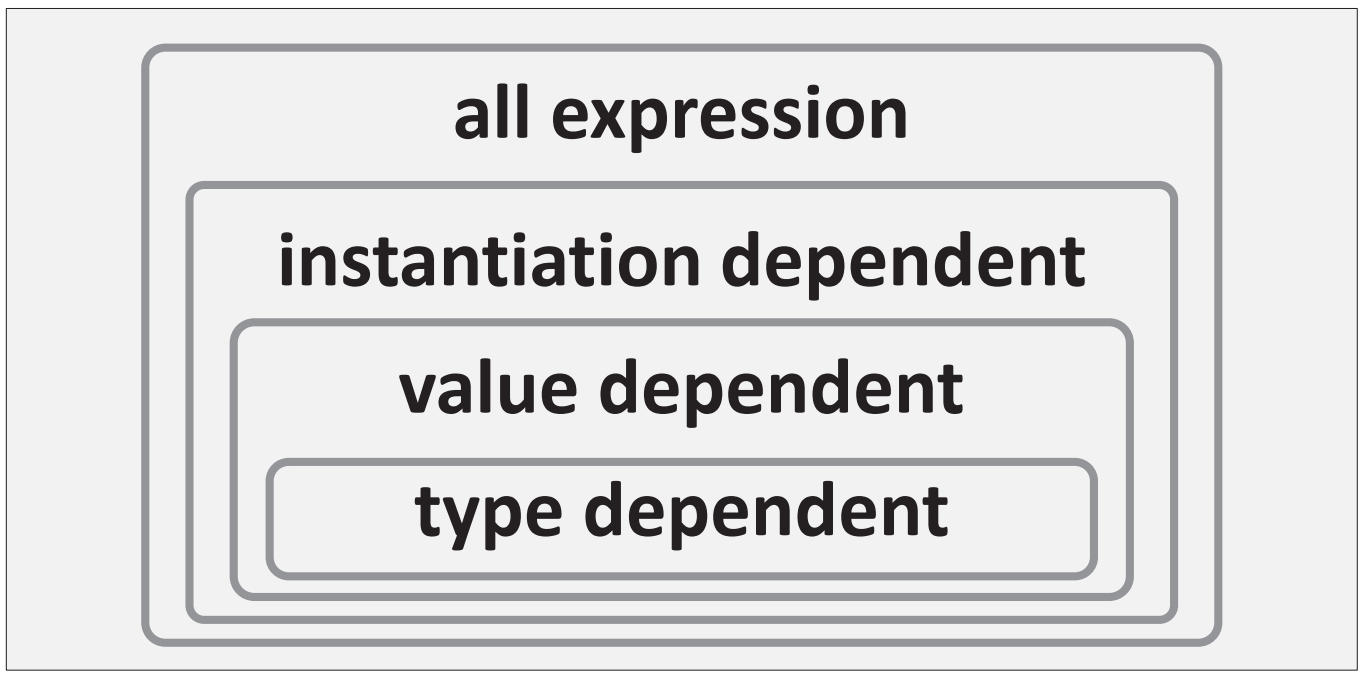
\includegraphics[width=0.8\textwidth]{part2/ch13/images/1.png} \\
图13.1. 类型、值和实例化型依赖表达式之间的关系
\end{center}

当从最内部的上下文(依赖于类型的表达式)到最外部的上下文时,模板的更多行为是在模板解析时决定的,因此不能在一个实例化到下一个实例化时进行变化。若f(x)中的x依赖于类型,那么f依赖于名称,需要进行两阶段查找(第14.3.1节),而若x依赖于值但不依赖于类型,那么f是不非依赖名称,在解析模板时可以完全确定其查找名称。

\subsection{编译错误}

当所有模板实例都会产生错误时,C++编译器允许(但不是必需的!)在解析模板时诊断错误。让我们扩展上一节中的f(x)例子来进一步探讨这个问题:

\begin{cpp}
void f() { }

template<int x> void nondependentCall() {
	f(x); // x is value-dependent, so f() is nondependent;
	// this call will never succeed
}
\end{cpp}

这里,调用f(x)在每个实例中都会产生错误,因为f是一个非依赖名称,而且唯一可见的f不接受参数。C++编译器在解析模板时会产生错误,或者会等到第一个模板实例化时才会产生错误:即使在这个简单的例子中,常用编译器的表现也会有所不同。可以构造相似的例子:表达式是实例依赖的,但并不是值依赖的。

\begin{cpp}
template<int N> void instantiationDependentBound() {
	constexpr int x = sizeof(N);
	constexpr int y = sizeof(N) + 1;
	int array[x - y]; // array will have a negative size in all instantiations
}
\end{cpp}











